\documentclass[12pt]{article}
\usepackage[arabic]{babel}
\usepackage[utf8]{inputenc}
\usepackage{amssymb}
\usepackage{geometry}
\usepackage{graphicx}
\usepackage{wrapfig}
\usepackage{amsmath}
\usepackage{lipsum}
\usepackage{caption}
\usepackage{ulem}
\usepackage{xcolor}
\usepackage{polyglossia}
\usepackage{tikz}
\usetikzlibrary{arrows.meta, positioning, shapes}
\setdefaultlanguage{arabic}
\setotherlanguage{english}

% Font and layout settings
\newfontfamily\arabicfont[Script=Arabic,Scale=1.2]{Amiri}
\geometry{top=2cm, bottom=2cm, left=2cm, right=2cm}

% Colors
\definecolor{titleColor}{HTML}{800000} % Maroon for titles
\definecolor{sectionColor}{HTML}{4682B4} % SteelBlue for sections
\definecolor{textHighlight}{HTML}{DAA520} % Goldenrod for highlights
\definecolor{backgroundColor}{HTML}{F0F8FF} % AliceBlue background
\definecolor{emphasisColor}{HTML}{228B22} % ForestGreen for emphasis

\begin{document}

\begin{center}
	{\Huge\textbf{\textcolor{titleColor}{ تأملات الصباح: استرجاع الذاكرة ورؤى المستقبل  }}}

    \vspace{0.5cm}
    
    \textbf{\textcolor{emphasisColor}{بابكر عثمان}} \\
    \vspace{0.2cm}
    \today
\end{center}

\section{التأمل والاتصال بالذات}
حديث الصباح دائمًا يحمل طاقة إيجابية وبداية هادئة لليوم. لنتحدث عن التأمل وما يمكن أن يجلبه من عمق واتصال بالذات، خصوصًا إذا اقترن بالأمل والرؤية العميقة.  
التأمل يُعتبر نافذة إلى الداخل، حيث يمكن للإنسان أن يتواصل مع مصادره الداخلية ويتحرر من التشويش. هو الوقت الذي يمكن فيه للإنسان أن يعيد ترتيب أفكاره، ويجعل من قلبه بوابة للنور والأمل.

\section{الإلهام من العفاض وكرمكول}
نعم، فأنا ابن العفاض. ألهمني فيديو هذا الصباح عن الكاتب العالمي \textbf{الطيب صالح}، وهو ابن منطقتنا العفاض وكرمكول، تلك المنطقة التي يحتضنها منحنى النيل.  
يا لها من صدفة جميلة وإلهام رائع! الطيب صالح، ابن منطقتي العفاض، كان بحق علمًا أدبيًا عالميًا. قصصه تعكس بعمق الروح السودانية والتجربة الإنسانية بمختلف أبعادها.  

\section{تأثير الطيب صالح}
ومن خلال عدسة الطيب صالح، يطل علينا عالم من العمق الإنساني. يتجاوز أدبه حدود الزمان والمكان، مسلطًا الضوء على صراعات الهوية والانتماء.  
هو الذي كتب عن السودانيين، عن أرواحهم المتعطشة للحرية والسلام، عن العادات والتقاليد التي تنمو في ظل صراع الهوية.

\section{كوش والحضارة القديمة}
تحتضن كوش ذاكرة الحضارة القديمة التي شهدت عبق التاريخ وتنوع الثقافات. كوش لم تكن مجرد حضارة، بل كانت دليلًا على قدرة البشر على الابتكار والاستدامة.  

% Title
\begin{center}
    {\Huge\textbf{\color{titleColor} الفكي قيلي: العالم المتجول في شمال السودان}}  
    \vspace{0.5cm}
\end{center}

\section*{\color{sectionColor} النسب العائلي}
\begin{itemize}
    \item \textbf{بابكر، مالك، عثمان، علي، الشيخ، محمود}
    \item \textbf{الفكي قيلي، مالك، مدني، عبدالرحمن، أبو القاسم، حميدة، حمد، حميدة، سراج، مصباح، سليم، رباط، غلام الله، عائد}
    \item \textbf{مقبول، أحمد الزيلعي، محمود، هاشم، مختار، علي العسكري، محمد، أبو القاسم، محمد الزامل، إسماعيل}
    \item \textbf{أحمد التقي، محمد النقي، علي الرضا، موسى الكاظم، جعفر الصادق، محمد الباقر، زين العابدين علي، الحسين، بن علي كرم الله وجهه، والسيدة فاطمة الزهراء بنت رسول الله صلى الله عليه وسلم}
\end{itemize}

\section*{\color{sectionColor} نبذة تاريخية عن الفكي قيلي}
هو \textbf{\color{emphasisColor} الفكي قيلي} صاحب القبة الموجودة حاليًا في \textbf{العفاض}، حيث درس الفقه وحفظ القرآن على يد جده \textbf{مدني}.  

في فترة الحكم التركي، طلب الأتراك من جده الفكي قيلي الحضور إلى تركيا ليكون ضمن علماء البلاط التركي وديوان الإفتاء، لكنه فضل البقاء في \textbf{السودان}، متجولًا في شمال البلاد لنشر العلوم الدينية وتعليم الفقه في مناطق عديدة.



\begin{wrapfigure}{r}{0.4\textwidth}
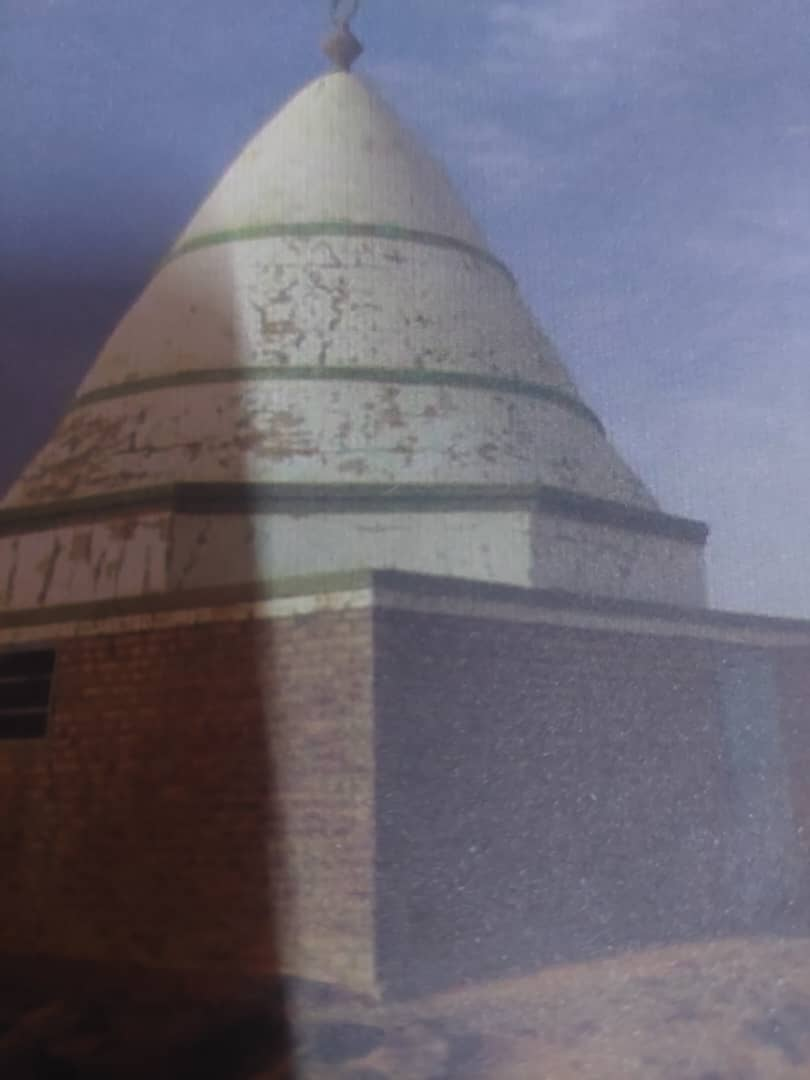
\includegraphics[width=0.4\textwidth]{y5.jpg}
\end{wrapfigure}



\begin{english}
\begin{center}
{\Huge\textbf{\textcolor{titleColor}\english{The Role of Sufi Orders in Sudan }}} \\
\end{center}

The Sufi orders have played a significant cultural and economic role in the lives of people in Sudan. Thanks to them, the social fabric has held together for centuries, achieving national unity through their influence. An example of this is our great ancestor, Sheikh Gili Wad Malik, who inherited the Qadiri Sufi lineage from his grandfather, Hamida the Great, the disciple of Gulamullah bin A'id. Tribes gathered around them, life stabilized, and social harmony was achieved. How much we need today to draw inspiration from this heritage and connect our turbulent present with our bright past.

\end{english}

\vspace{.2cm}

\begin{arabtext}
{ \hspace{.1cm} للطرق الصوفية دور ثقافى واقتصادى كبير فى حياة الناس فى السودان، وبفضلهم تماسك النسيج الاجتماعى لقرون طويلة، وتحققت الوحدة الوطنية من خلالها. ومثال لذلك جدنا الاكبر الفكى قيلي ود مالك الذى ورث السجادة القادرية من جده حميدة الكبير حفيد غلام الله بن عائد. حولهم التفت القبائل واستقرت الحياة، وتحقق السلم الاجتماعى. ما احوجنا اليوم ان نستلهم التراث ونربط حاضرنا المضطرب بماضينا المشرق.}
\end{arabtext}
\begin{wrapfigure}{r}{0.4\textwidth}
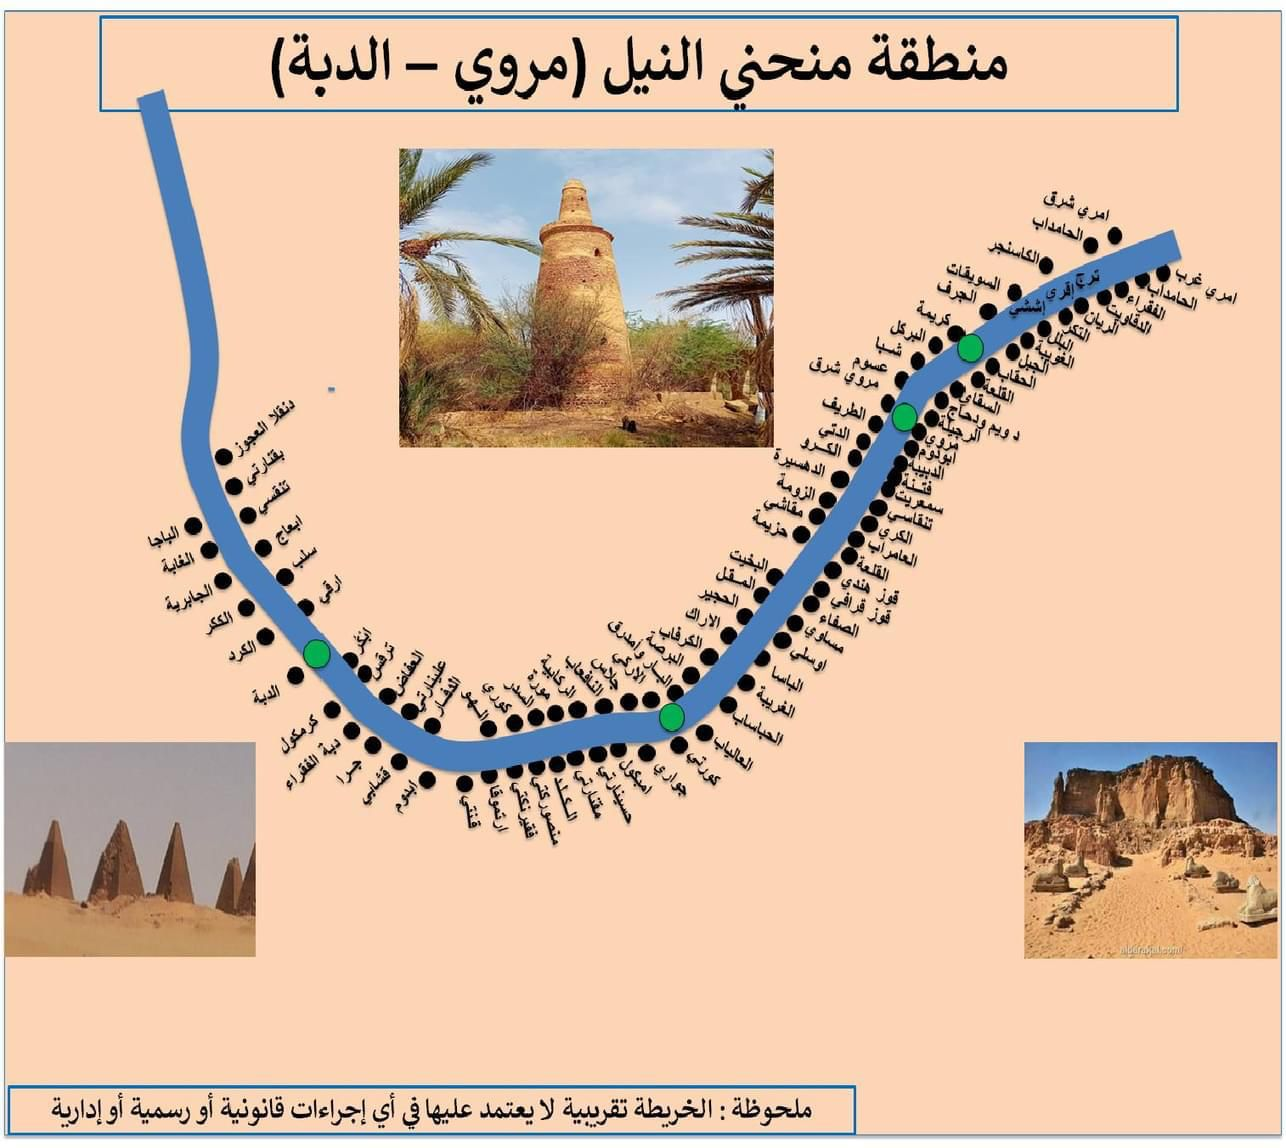
\includegraphics[width=0.4\textwidth]{120.jpg}
\end{wrapfigure}

\section{نحو سودان جديد}
إنني أرى في كل هذه العناصر حافزًا لبناء \textbf{سودان جديد}، يتمتع بالطمأنينة والسلام، حيث ينمو الوعي الجماعي كقوة دافعة للتغيير.  
يجب أن نستعيد تلك الروح المشتركة، ونتذكر أننا جميعًا جزء من نسيج واحد. عبر التعليم والتثقيف، يمكننا تعزيز قيم السلام والمحبة، وبناء جسور من الفهم بين الثقافات المختلفة.  

\section{رحلتي العلمية}
بدأت رحلتي العلمية في كلية الطب البيطري بجامعة الخرطوم، حيث أكملت دراستي للبكالوريوس والماجستير.  
ثم انتقلت إلى \textbf{Wye College} في المملكة المتحدة، والتي كانت محطة فارقة في مسيرتي الأكاديمية والبحثية، حيث انفتحت لي آفاق جديدة لاستكشاف تقنيات وأساليب حديثة.

\section{من الريف الإنجليزي إلى بناء التماسك في السودان}
أتذكر بوضوح دراستي للدكتوراه في \textbf{Wye College}، التي كانت جزءًا من جامعة لندن. الريف الإنجليزي حول الكلية كان يتميز بجماله الطبيعي الهادئ، مما وفر لي بيئة مثالية للتأمل والدراسة العميقة.

\section{بحثي في جين البورولا}
درستُ إدخال \textbf{جين البورولا} في أغنام \textbf{Romney}، وكان هذا البحث هو الأول من نوعه في المملكة المتحدة.  
فتح هذا البحث آفاقًا جديدة لدراسة الصفات المعقدة التي كان يُعتقد أنها تخضع لتحكم العديد من الجينات.  
كانت هذه الدراسة خطوة مهمة في علم الوراثة، حيث أثبتت كيف يمكن لجين واحد أن يؤثر على صفات كانت تُعتبر متعددة الجينات.

\section{إنشاء المنصة الرقمية المتكاملة}
كجزء من جهودنا لتحقيق التماسك والتنمية المستدامة، قمنا بإنشاء \textbf{منصة رقمية متقدمة} تعتمد على الذكاء الاصطناعي، والحوسبة السحابية، والتقنيات الحيوية لدعم الأبحاث والمشاريع الاجتماعية.  
تهدف هذه المنصة إلى توفير بيئة تفاعلية لتحليل البيانات الضخمة، ومحاكاة النماذج المعقدة، وتعزيز التعاون بين الباحثين والمجتمعات المتضررة.

\section{الانتقال إلى الأدوات الحديثة}
لقد تطورت أساليب عملي لتشمل \textbf{LaTeX}، مُقدِّرًا قوته في تنسيق الوثائق، مما وفر لي أدوات مثالية لتنظيم الأفكار وعرضها بوضوح.  
كما أنني تبنيت تقنيات جديدة في تحليل البيانات، مما ساعدني على تقديم رؤى أكثر دقة وعمقًا.

\section{\textcolor{sectionColor}{المفهوم الأساسي للمنصة}} المنصة الإلكترونية الرقمية تُعتبر الوسيلة الأساسية لتحقيق أهداف المشروع. ستكون بمثابة نقطة التقاء للمعرفة، والتفاعل، والمشاركة بين الأفراد والمجتمعات. من خلال هذه المنصة، يمكن تعزيز الوعي الجماعي وبناء بيئة من التعاون والتفاهم.
\section{\textcolor{sectionColor}{رؤى المستقبل}}
إن استرجاع الذاكرة وربطها برؤى المستقبل هو جوهر رحلتي العلمية والإنسانية.  
من خلال التأمل في تجاربي والاندماج مع مجتمعي، أسعى إلى المساهمة في بناء مستقبل أفضل، حيث يكون \textbf{العلم والتماسك المجتمعي} هما الركيزتان الأساسيتان للتنمية المستدامة.




\begin{center}
    {\Huge\textbf{\textcolor{titleColor}{ السودان  الحرب والسلام الاستقرار والازدهار }}}
    \vspace{0.5cm}

    \textbf{\textcolor{emphasisColor}{بابكر عثمان}} \\
    \vspace{0.2cm}
    \today
\end{center}

مؤشرات لبنان السياسية جلسة النواب وانتخاب الرئيس من المؤسسة العسكرية قد تشير الى توجه مماثل فى السودان: جيش واحد يحتكر السلاح وتشجيع تيار وطنى ديمقراطى يبتعد عن الحروب ويركز على استقرار وازدهار البلد وطى صفحة ايران وحزب الله والى الابد. ما طرحته يعكس تطلعات مشروعة نحو الاستقرار والازدهار، سواء في لبنان أو السودان. فكرة جيش وطني موحد يحتكر السلاح ويعمل على حماية السيادة بعيداً عن التدخلات الخارجية والصراعات الداخلية هي خطوة جوهرية نحو بناء دولة قوية ومستقرة.

تشجيع تيار وطني ديمقراطي يركز على تنمية المجتمع بدلاً من الدخول في حروب وصراعات سياسية قد يكون المفتاح لتحقيق هذا الهدف. بالنسبة لطوي صفحة التدخلات الخارجية، مثلما ذكرت عن إيران وحزب الله، فهو أمر يتطلب توافقاً داخلياً وإرادة شعبية وسياسية، خصوصاً أن التدخلات الخارجية عادةً ما تجد موطئ قدم في الدول التي تعاني من الانقسامات الداخلية. أما في السودان، فالوضع مشابه إلى حد ما، حيث إن الجيش الوطني الموحد والتوجه نحو التنمية بدلاً من الصراعات القبلية والحروب الداخلية يمكن أن يكون حلاً مستداماً للخروج من الأزمات. نسأل الله أن يتحقق هذا النموذج في بلدك وفي كل البلدان التي تعاني من الأزمات، وأن يعم السلام والاستقرار الجميع.

\section*{نقاش أعمق حول الموضوع}

\subsection*{1. احتكار الجيش للسلاح: رؤية استراتيجية أم تحديات؟}
احتكار الجيش للسلاح هو خطوة أساسية لضمان الأمن القومي وتفادي الفوضى الناتجة عن تعدد المليشيات أو الجماعات المسلحة. ولكن هذا المفهوم يتطلب:
\begin{itemize}
    \item إعادة هيكلة الجيش ليصبح جيشًا قوميًّا يمثل جميع مكونات الشعب، مما يقلل من احتمالية احتكار السلطة لفئة واحدة.
    \item إعادة تأهيل المليشيات أو دمجها في الجيش وفق شروط وطنية صارمة تضمن الولاء للدولة فقط.
    \item دور المجتمع الدولي في دعم هذا التوجه من خلال الضغط على الأطراف التي تغذي الصراعات، وضمان تطبيق معايير حقوق الإنسان في أداء الجيش.
\end{itemize}

في حالة لبنان، نجد أن وجود حزب الله كمليشيا مسلحة يعتبر عقبة رئيسية أمام بناء دولة مستقرة، حيث يتداخل دوره كجماعة مسلحة مع دوره السياسي، مما يعطل بناء جيش موحد. السودان يواجه تحديات مشابهة مع وجود مليشيات مثل قوات الدعم السريع التي تنافس الجيش.

\subsection*{2. التيار الوطني الديمقراطي: فرصة تاريخية أم معضلة واقعية؟}
التيارات الوطنية الديمقراطية في البلدان التي تعاني من الصراعات عادة ما تواجه تحديات هائلة، مثل ضعف الدعم الشعبي نتيجة قلة الوعي السياسي أو ضغط التيارات المتطرفة. لكي ينجح هذا التيار، يجب أن يكون له مشروع وطني واضح يتجاوز الخلافات الإيديولوجية ويركز على قضايا أساسية مثل الاقتصاد، التعليم، والصحة. تجربة السودان بعد الثورة تشير إلى أن هناك فرصة حقيقية لتشكيل تيار وطني ديمقراطي، لكن النزاعات السياسية بين المدنيين والعسكريين أضعفت هذا التوجه.

\subsection*{3. التخلص من النفوذ الخارجي: حلم بعيد أم ضرورة قريبة؟}
التدخلات الخارجية غالبًا ما تُغذى من فراغات سياسية داخلية، لذلك:
\begin{itemize}
    \item الاستقلالية السياسية تبدأ من الداخل، أي بوجود حكومة قوية تمتلك شرعية شعبية وإرادة واضحة.
    \item يجب أن تكون هناك شراكات دولية متوازنة لا تسمح لطرف خارجي بالتفوق على حساب مصلحة البلد.
\end{itemize}

لبنان يعاني من تدخلات مباشرة من إيران عبر حزب الله، فيما السودان كان ولا يزال ساحة لتدخلات إقليمية ودولية، مثل تدخلات مصر، الإمارات، وقطر، ما يعقّد المشهد.

\subsection*{4. المستقبل: هل يمكن تحقيق هذه الرؤية؟}
يمكن للبنان أن يخطو نحو هذا الاتجاه إذا حدث توافق داخلي على تحييد السلاح خارج إطار الدولة، لكن هذا يتطلب وقتًا وإرادة سياسية قوية. السودان يمتلك فرصة حقيقية إذا تم تسريع عملية التحول الديمقراطي، خاصة بعد تقليص نفوذ المليشيات وعودة الروح المدنية للقيادة السياسية. 

\section*{خاتمة}
نجاح هذه الرؤية يعتمد على إرادة الشعوب والنخب السياسية، بجانب دور المجتمع الدولي في الحد من التدخلات الخارجية. التحديات كثيرة، لكنها ليست مستحيلة. 

\section*{المعضلة الاقتصادية والتنموية في السودان}
صحيح تمامًا، معضلة التنمية في السودان، أو أي بلد يعاني من أزمات مشابهة، ترتبط ارتباطًا وثيقًا بتوفير دعم مادي ضخم وتوجيهه بشكل متوازن وفعّال. لتفجير قلاع الإنتاج وتحقيق تنمية مستدامة، نحتاج إلى معالجة شاملة تجمع بين الداخل والخارج. يمكن تحليل القضية من عدة أبعاد:

\subsection*{1. دعم القوى الدولية والإقليمية: ضرورة تكاملية}
ضمان تحقيق تنمية حقيقية في السودان، يجب إشراك القوى الدولية والإقليمية المعنية بمصالح السودان. لكن هذا الدعم يجب أن يكون مبنيًا على:
\begin{itemize}
    \item شراكات عادلة: بحيث لا تتحول المساعدات أو الاستثمارات إلى أداة للهيمنة أو فرض أجندات سياسية.
    \item مبادرات تنموية مستدامة: التركيز على مشروعات البنية التحتية، الزراعة، والطاقة بدلًا من المساعدات الإنسانية قصيرة المدى.
    \item توجيه الدعم للقطاعات المنتجة: مثل الزراعة، الثروة الحيوانية، التعدين، والتكنولوجيا، بدلًا من اقتصار الدعم على الاستهلاك.
\end{itemize}

مثال عملي:
\begin{itemize}
    \item يمكن لدول الخليج، التي لها مصالح اقتصادية في السودان، دعم الزراعة والإنتاج الغذائي الذي يعود بالنفع على الطرفين.
    \item الدول الغربية، مثل الولايات المتحدة والاتحاد الأوروبي، يمكنها التركيز على تمويل الطاقة النظيفة والتعليم.
\end{itemize}

\subsection*{2. توجيه الدعم إلى الداخل: ضمان التوازن وعدالة التوزيع}
الدعم الخارجي وحده ليس كافيًا؛ يجب توجيه الموارد إلى الداخل بشكل عادل وفعّال:
\begin{itemize}
    \item تعزيز اللامركزية: لضمان وصول التنمية إلى المناطق المهمشة مثل دارفور، النيل الأزرق، وكردفان.
    \item تمكين الشباب والمرأة: باعتبارهم العمود الفقري لقلاع الإنتاج في المستقبل.
    \item إصلاح النظام المالي والإداري: لضمان عدم تسرب الدعم إلى الفساد أو استغلاله في نزاعات سياسية.
\end{itemize}

مثال عملي:
\begin{itemize}
    \item إنشاء صندوق سيادي تحت رقابة دولية لإدارة الدعم المادي والاستثمار في مشاريع كبرى.
    \item تشجيع القطاع الخاص السوداني على لعب دور أكبر في التنمية، مع توفير تسهيلات وقروض.
\end{itemize}

\subsection*{3. تفجير قلاع الإنتاج: خطوة عملية للنهوض الاقتصادي}
السودان يمتلك إمكانيات هائلة إذا تم توظيفها بشكل صحيح:
\begin{itemize}
    \item الزراعة: السودان معروف بسلة غذاء العالم؛ يمكن تحويل الزراعة إلى قطاع صناعي متطور بالاعتماد على التكنولوجيا والابتكار.
    \item التعدين: الاستفادة من الثروات الطبيعية مثل الذهب والمعادن بشكل عادل ودون استغلال خارجي.
    \item الطاقة: تطوير مصادر الطاقة التقليدية والاعتماد على الطاقة الشمسية والرياح لتوفير بيئة إنتاج مستدامة.
\end{itemize}

\subsection*{4. الحل السياسي والتنمية: علاقة متبادلة}
لا يمكن فصل التنمية الاقتصادية عن الحل السياسي. أي دعم خارجي لن يثمر إلا في بيئة سياسية مستقرة.
\begin{itemize}
    \item إعادة بناء الثقة بين الأطراف السياسية: لتحقيق استقرار سياسي طويل الأمد.
    \item وقف النزاعات المسلحة: وتوجيه الإنفاق العسكري إلى التنمية.
    \item تعزيز المصالحة الوطنية: لضمان مشاركة جميع السودانيين في عملية البناء.
\end{itemize}

\subsection*{5. توحيد القوى الدولية والإقليمية: استثمار المصالح المشتركة}
يمكن تحقيق هذا الهدف من خلال مبادرات تشمل:
\begin{itemize}
    \item قمم إقليمية تجمع السودان والدول ذات المصالح المشتركة مثل دول الخليج، مصر، والاتحاد الأوروبي.
    \item مشروعات مشتركة: مثل مشروعات الربط الكهربائي مع إثيوبيا أو ممرات تجارية مع مصر.
    \item دبلوماسية اقتصادية نشطة: لإقناع القوى الكبرى بربط مصالحها مع ازدهار السودان، بدلًا من الصراعات عليه.
\end{itemize}

\section*{ختامًا: السودان كنموذج للإصلاح الشامل}
الربط بين القوى الدولية، التنمية الاقتصادية، والحل السياسي ليس مهمة سهلة، لكنه أمر ضروري لتفجير قلاع الإنتاج وتحقيق الاستقرار. السودان يمكن أن يكون نموذجًا للإصلاح الشامل إذا تم استغلال موقعه الجغرافي، موارده الطبيعية، وتراثه الثقافي في مشروع وطني متكامل.



\section{مصر وإثيوبيا: الصراع حول مياه النيل وسد النهضة}
الصراع بين مصر وإثيوبيا حول مياه النيل وسد النهضة يعكس مدى أهمية السودان كطرف في توازن القوى المائية.

\section{دول الخليج وتركيا}
تسعى كل من السعودية، الإمارات، وقطر إلى تعزيز نفوذها في السودان، حيث ينقسم الدعم بين أطراف سياسية متنافسة.

\section{إيران وإسرائيل}
لعبت إيران دورًا في دعم جماعات معينة في السودان سابقًا، بينما تسعى إسرائيل لتقليل النفوذ الإيراني وبناء علاقات مع السودان عبر التطبيع.

\section{التدخلات الدولية: أدوات للتنافس على النفوذ}
\subsection{الصين}
السودان يعتبر جزءًا من مبادرة "الحزام والطريق"، حيث تستثمر الصين في البنية التحتية والنفط.

\subsection{الولايات المتحدة}
تسعى الولايات المتحدة لتحقيق استقرار سياسي يخدم مصالحها، لكنها تواجه تحديًا بسبب تنافسها مع الصين وروسيا.

\subsection{روسيا}
تركز روسيا على تعزيز وجودها العسكري في البحر الأحمر واستغلال الموارد المعدنية.

\section{تداعيات المنافسة على السودان}
\subsection{استمرار عدم الاستقرار}
التدخلات الخارجية تغذي الصراعات الداخلية عبر دعم أطراف مختلفة.

\subsection{ضعف التنمية}
معظم الاستثمارات الخارجية تركز على استغلال الموارد بدلاً من بناء اقتصاد متنوع ومستدام.

\subsection{إضعاف السيادة}
تتحول الحكومات السودانية إلى أدوات بيد القوى الإقليمية والدولية، ما يجعل القرارات الوطنية مرهونة للمصالح الخارجية.

\section{كيف يمكن مواجهة الأطماع؟}
\subsection{تعزيز الوحدة الوطنية}
يجب أن تعمل الحكومة السودانية على بناء توافق داخلي قوي بين القوى السياسية لضمان عدم استغلال الخلافات من قبل الخارج.

\subsection{تنويع الشراكات}
الاعتماد على شريك دولي واحد يعرض البلاد للهيمنة، لذلك يجب تنويع العلاقات مع قوى متعددة لتحقيق توازن.

\subsection{إصلاح النظام الاقتصادي}
تقليل الاعتماد على المساعدات الخارجية من خلال تطوير القطاعات المحلية مثل الزراعة والتعدين.

\subsection{استراتيجية إقليمية متوازنة}
السودان يجب أن يلعب دورًا محوريًا كجسر للتعاون بدلاً من أن يكون ساحة للصراعات الإقليمية.

\subsection{الاستثمار في الشعب}
بناء قدرات الشباب والمرأة يمكن أن يكون أداة فعالة لمواجهة الأطماع الخارجية عبر تعزيز الإنتاجية الداخلية.

\section{ختامًا: السودان بين الأطماع والفرص}
السودان يمتلك فرصة تاريخية لتحويل المنافسة الإقليمية والدولية إلى ميزة إذا تمكن من بناء استراتيجية وطنية شاملة. السؤال الآن: هل يمكن للسودانيين تجاوز الخلافات الداخلية لتحقيق هذا الهدف؟ الإجابة على السؤال تتطلب واقعية ورؤية تحليلية عميقة: هل يمكن للسودانيين تجاوز الخلافات الداخلية لتحقيق هذا الهدف؟

\section{التحديات الكبرى التي تواجه السودانيين}
\subsection{الانقسامات الداخلية}
السودان يعاني من تنوع عرقي وثقافي وديني يُستخدم أحيانًا كأداة لتأجيج الصراعات بدلاً من كونه مصدرًا للثراء الوطني.

\subsection{الإرث التاريخي للنزاعات}
عقود من الحروب الأهلية والنزاعات المسلحة أضعفت النسيج الاجتماعي وزرعت عدم الثقة بين المكونات المختلفة.

\subsection{الضعف المؤسسي}
الدولة السودانية تعاني من ضعف في مؤسساتها نتيجة التدخلات العسكرية المتكررة والفساد المزمن.

\subsection{التدخلات الخارجية}
القوى الإقليمية والدولية غالبًا ما تسعى لتعظيم مصالحها على حساب مصلحة السودان الوطنية، مما يعقّد أي جهود داخلية للإصلاح.

\section{مؤشرات الأمل والإمكانات المتاحة}
\subsection{وعي شعبي متزايد}
السودانيون أظهروا وعيًا سياسيًا متقدمًا خلال ثورة ديسمبر 2018، حيث أثبتوا قدرتهم على تنظيم احتجاجات سلمية وضغط شعبي نحو التغيير.

\subsection{الموارد الطبيعية}
السودان غني بالموارد الزراعية، المعدنية، والبشرية، مما يمنحه قاعدة قوية إذا تم استغلالها بشكل عادل وفعّال.

\subsection{الدور الشبابي والنسائي}
الشباب والنساء لعبوا دورًا كبيرًا في الحراك الشعبي، ويمكن أن يكونوا القوة الدافعة نحو بناء مستقبل جديد.

\section{متطلبات تجاوز الخلافات}
\subsection{بناء عقد اجتماعي جديد}
يجب الاتفاق على رؤية وطنية مشتركة تحترم التنوع وتضمن حقوق جميع السودانيين.

\subsection{إصلاح المؤسسات}
إنشاء مؤسسات قوية وشفافة تكون محايدة وخاضعة للمساءلة لضمان توزيع عادل للسلطة والثروة.

\subsection{التعليم والتوعية}
الاستثمار في التعليم لتعزيز قيم المواطنة والوعي السياسي، مما يساعد في تقليل التلاعب الخارجي والخلافات الداخلية.

\subsection{تحقيق العدالة الانتقالية}
معالجة مظالم الماضي من خلال آليات عدالة انتقالية تعيد بناء الثقة بين مختلف مكونات المجتمع.

\subsection{استراتيجية تنموية وطنية}
توجيه الموارد نحو مشروعات تنموية كبرى تعزز الاقتصاد وتخلق فرص عمل، مما يقلل من أسباب الصراعات.

\section{هل السودانيون قادرون؟}
\subsection{الإجابة المختصرة: نعم، لكن بشروط}
السودانيون أثبتوا عبر التاريخ أنهم شعب resilient قادر على مواجهة التحديات الكبرى. لكن تجاوز الخلافات يحتاج إلى قيادة رشيدة، إرادة سياسية صادقة، ودعم مجتمعي عميق.

إذا تمكن السودانيون من تحويل تنوعهم إلى قوة، واستخدام الموارد بحكمة، وتحييد التدخلات الخارجية، فسيكون بمقدورهم ليس فقط تجاوز الخلافات، بل أيضًا بناء نموذج يُحتذى به للتعايش والتنمية في المنطقة.

\section{صياغة رؤية متكاملة للنموذج المثالي للسودان المستقبلي}
يمكن بناء الرؤية على الأعمدة الأربعة التي ذكرتها: الثراء في التنوع، القيادة الرشيدة، الوعي المجتمعي العميق، والتنمية الشاملة.

\subsection{الثراء في التنوع: السودان كفسيفساء موحدة}
\subsubsection{التنوع كمصدر قوة}
السودان بلد متعدد الثقافات، الأعراق، والأديان. بدلاً من أن يكون هذا التنوع مصدرًا للفرقة، يمكن أن يتحول إلى عامل ثراء حضاري واقتصادي من خلال:
\begin{itemize}
    \item تعزيز ثقافة الحوار والتعايش.
    \item تسليط الضوء على الإرث الثقافي المشترك والتقاليد السودانية الجامعة.
    \item دعم الفنون والآداب التي تحتفي بالتنوع وتعكس الهوية السودانية المتكاملة.
\end{itemize}

\subsubsection{التنوع الاقتصادي}
استغلال الموارد الطبيعية والزراعية بشكل متوازن لتلبية احتياجات كافة الأقاليم والمناطق، مع ضمان عدالة التوزيع.

\subsubsection{النموذج المثالي}
أن يُصبح السودان منارة إقليمية تحتفي بتعددها، وتصدر للعالم نموذجًا لكيفية التعايش بين المختلفين.

\subsection{القيادة الرشيدة: مفتاح التغيير الحقيقي}
\subsubsection{قيادة واعية ومسؤولة}
تعمل من أجل الوطن لا من أجل مصالح شخصية أو حزبية.
\begin{itemize}
    \item تمتلك رؤية استراتيجية طويلة الأمد لبناء دولة حديثة.
    \item تعتمد على الكفاءة والشفافية في اختيار المسؤولين وإدارة الموارد.
\end{itemize}

\subsubsection{القيادة التحويلية}
تعزيز فكرة القائد كخادم للشعب، لا سيد عليه.
\begin{itemize}
    \item تمكين القيادات الشابة والمرأة للمشاركة في صنع القرار.
    \item بناء مؤسسات وطنية قوية تكون فوق الأفراد والأحزاب.
\end{itemize}

\subsubsection{النموذج المثالي}
قيادة تُعيد الثقة بين المواطن والدولة، وتجعل من السودان مثالًا في الحكم الرشيد بإفريقيا والمنطقة.



\section{3. الوعي المجتمعي العميق: الأساس لبناء وطن مستدام}
\subsection{التعليم كأولوية}
\begin{itemize}
    \item بناء نظام تعليمي يركز على تعزيز قيم المواطنة والتنوع، ويركز على تنمية المهارات العملية.
    \item مكافحة الأمية، خاصة في المناطق الريفية والمهمشة.
\end{itemize}

\subsection{تعزيز المسؤولية المجتمعية}
\begin{itemize}
    \item حملات توعية شاملة لبناء وعي سياسي واقتصادي لدى المواطنين.
    \item دعم المبادرات المحلية التي تعزز الانتماء الوطني وتدعم التنمية.
\end{itemize}

\subsection{التواصل الشعبي}
\begin{itemize}
    \item إشراك المجتمعات المحلية في صنع القرار والتنمية.
    \item إحياء دور النقابات والاتحادات كصوت مجتمعي فاعل.
\end{itemize}

\subsection{النموذج المثالي}
شعب واعٍ يشارك في بناء الدولة ويقف في وجه أي محاولات لزرع الفرقة أو التلاعب بالمصالح الوطنية.

\hrule

\section{4. التنمية الشاملة: البنية التحتية والاقتصاد في قلب المشروع الوطني}
\subsection{اقتصاد متوازن ومستدام}
\begin{itemize}
    \item تنمية قطاعات الزراعة، التعدين، والطاقة لتحقيق الاكتفاء الذاتي والتصدير.
    \item جذب الاستثمارات الأجنبية بشروط وطنية عادلة.
    \item دعم الشركات الناشئة والابتكار، خاصة في التكنولوجيا والصناعات الإبداعية.
\end{itemize}

\subsection{البنية التحتية المتكاملة}
\begin{itemize}
    \item تطوير الطرق، السكك الحديدية، وشبكات الاتصالات لربط كافة أنحاء البلاد.
    \item تحسين الخدمات الأساسية مثل الصحة والمياه والكهرباء لتكون متاحة للجميع.
\end{itemize}

\subsection{الاستدامة البيئية}
\begin{itemize}
    \item حماية الموارد الطبيعية.
    \item اعتماد سياسات طاقة نظيفة ومشروعات تنموية تحافظ على البيئة.
\end{itemize}

\subsection{النموذج المثالي}
أن يُصبح السودان دولة منتجة ذات اقتصاد قوي ومتنوع، تتصدر مؤشر التنمية المستدامة في إفريقيا.

\hrule

\section{ختامًا: السودان كنموذج ملهم للعالم}
السودان المثالي هو وطن يحتفي بثروته في تنوعه، تديره قيادة رشيدة بحكمة ومسؤولية، مدعومًا بوعي مجتمعي عميق، وقائمًا على اقتصاد قوي وتنمية شاملة. هذا النموذج لن يكون فقط طريقًا للنهوض بالسودان، بل قد يُلهم العديد من الدول التي تواجه تحديات مشابهة. 

إقناع الآخرين، سواء كانوا داخليين أو خارجيين، يتطلب استراتيجيات مدروسة ترتكز على المصداقية، الإقناع بالحجة، وخلق المصالح المشتركة. بالنظر إلى أن مواقف بعض الأطراف كانت مخيبة للآمال منذ ثورة ديسمبر، فإن إعادة بناء الثقة وإشراكهم في مشروع وطني جامع يجب أن تكون أولوية.

\hrule

\section{أولًا: التعامل مع الأطراف الداخلية}
\subsection{1. إعادة بناء الثقة بين الأطراف المختلفة}
\begin{itemize}
    \item فتح حوار وطني شامل: إطلاق حوار مفتوح يشمل جميع القوى السياسية والاجتماعية، مع التركيز على القواسم المشتركة بدلاً من نقاط الخلاف.
    \item التأكيد على أن مصلحة السودان فوق جميع المصالح الفردية أو الفئوية.
\end{itemize}

\subsection{آليات العدالة الانتقالية}
\begin{itemize}
    \item معالجة المظالم التي وقعت خلال الفترات السابقة بشفافية وعدالة لضمان عدم تكرارها.
    \item إظهار إرادة سياسية صادقة لتحقيق المصالحة الوطنية.
\end{itemize}

\subsection{2. خلق مصلحة مشتركة}
\begin{itemize}
    \item تقديم خطة تنموية واضحة تكون نتائجها ملموسة لجميع الأطراف.
    \item إشراك القوى المختلفة في تنفيذ المشاريع التنموية وإعطائهم أدوارًا عملية ومسؤوليات.
    \item ضمان التوزيع العادل للموارد والتنمية بين الأقاليم المختلفة.
\end{itemize}

\subsection{3. تعزيز الوعي المجتمعي}
\begin{itemize}
    \item إطلاق حملات توعية لشرح الرؤية الوطنية والمشروع التنموي بأسلوب بسيط ومباشر.
    \item استخدام الإعلام الوطني والرموز الثقافية والشخصيات المؤثرة لبناء الثقة وحشد الدعم.
    \item التركيز على الأجيال الشابة عبر التعليم وبرامج التدريب والتأهيل.
\end{itemize}

\hrule

\section{ثانيًا: التعامل مع الأطراف الإقليمية والدولية}
\subsection{1. توضيح أهمية الاستقرار السوداني للجميع}
\subsubsection{الإقليم:}
\begin{itemize}
    \item إبراز أن استقرار السودان يصب في مصلحة الأمن الإقليمي ومكافحة الإرهاب والحد من الهجرة غير...
\end{itemize}



\section{التأكيد على أن السودان يمكن أن يكون جسرًا للتعاون الاقتصادي بين الدول الإفريقية والعربية.}
\subsection{الدولية:}
\begin{itemize}
    \item شرح أن الاستقرار السوداني يمكن أن يُسهم في استقرار المنطقة بأكملها، مما يخفف الضغوط الدولية على قضايا اللاجئين والأمن.
\end{itemize}

\subsection{2. جذب الاستثمارات الدولية والإقليمية}
\begin{itemize}
    \item تقديم خطط استثمارية شفافة ومجزية في قطاعات مثل الزراعة، الطاقة، والبنية التحتية.
    \item ضمان توفير بيئة قانونية وسياسية مستقرة لجذب المستثمرين.
\end{itemize}

\subsection{3. الحياد في الصراعات الدولية والإقليمية}
\begin{itemize}
    \item اعتماد سياسة خارجية محايدة تقوم على مصلحة السودان أولًا.
    \item الابتعاد عن المحاور السياسية المتصارعة والعمل كطرف وسيط لبناء جسور التعاون.
\end{itemize}

\hrule

\section{ثالثًا: التعاطي مع الإحباط الناتج عن المواقف السابقة}
\subsection{1. تقييم الماضي بموضوعية}
\begin{itemize}
    \item الاعتراف بالأخطاء السابقة ومراجعة أسباب الإحباط التي حدثت منذ ثورة ديسمبر.
    \item وضع آليات تحول دون تكرار تلك الأخطاء، مثل الشفافية والمساءلة.
\end{itemize}

\subsection{2. بناء رؤية مستقبلية مقنعة}
\begin{itemize}
    \item تقديم رؤية واضحة ومحددة للمستقبل تستند إلى أرقام وخطط قابلة للتنفيذ.
    \item التركيز على المكاسب المشتركة لجميع الأطراف من تحقيق هذه الرؤية.
\end{itemize}

\subsection{3. إبراز النجاحات الصغيرة كبوادر تغيير}
\begin{itemize}
    \item التركيز على تحقيق إنجازات صغيرة لكنها ملموسة لتكون دليلًا على الجدية.
    \item استخدام هذه الإنجازات كبناء ثقة تدريجي مع الأطراف المختلفة.
\end{itemize}

\hrule

\section{رسالة الإقناع الأساسية}
"السودان وطننا جميعًا، ومصلحته هي مصلحتنا المشتركة. إذا توحدنا حول مشروع وطني تنموي، يمكننا أن نكون نموذجًا يُحتذى به للعالم. لن نحقق ذلك إلا بالتكاتف، الصدق، والاعتراف بأن الوطن أكبر من أي خلاف أو مصلحة شخصية."

\subsection{الإقناع يبدأ بالمصداقية والعمل الجاد، مع خلق بيئة يشعر فيها الجميع أن لديهم دورًا ومصلحة حقيقية في النجاح.}




\newpage  


\begin{center}                       {\Huge\textbf{\textcolor{titleColor}{ اطلاق منصة الكترونية لتعزيز السلام التعافى والتماسك تكنولوجيا }}}         
\end{center}
	\vspace{0.5cm}


\section {\textcolor{sectionColor}{المقدمة}}
أنا بابكر عثمان أكاديمي وباحث في مجالات متعددة تشمل البيولوجيا الوراثية، النظم البيولوجية، علوم البيانات، الحوسبة الحيوية، وعلوم القلب، وتطبيقاتها في الأمن الغذائي، التصنيع الدوائي، الطب الحيوي، والتماسك الفردي والمجتمعي. يسرني أن أطلق هذه المنصة الإلكترونية المتكاملة التي تهدف إلى تسريع تقدم المجتمعات من خلال توظيف التكنولوجيا الرقمية المتطورة.

\textbf{الهدف الرئيسي لهذه المنصة هو تحسين التواصل وتعزيز التعاون بين الأفراد، المجتمعات، والمنظمات المحلية والدولية في مختلف أنحاء العالم، سواء في الدول المتقدمة أو النامية.} هذه المنصة ستكون أداة فعالة لربط المجتمعات، وتحقيق التنمية المستدامة، وتعزيز السلام الاجتماعي من خلال استخدام تقنيات مثل \textLR{Artificial Intelligence} و \textLR{Big Data}.

كمتفرغ للعمل، أود إنشاء منصة إلكترونية معلوماتية خدمية تربط الأفراد والمجتمعات للقطاعات المختلفة تعتمد على البيانات وتقانة المعلومات للتحليل واتخاذ القرارات.
تشمل القطاعات المستهدفة:
\begin{itemize}
    \item \textbf{الأمن الغذائي}.
    \item \textbf{الصحة العامة والتصنيع الدوائي واتجاهات العلاج الحديثة للأمراض المستعصية}.
    \item \textbf{الموارد الطبيعية، البيئة، والمناخ}.
\end{itemize}
المنصة ستخدم قطاع الأدوية كمصدر للمعلومات وإدارة وتحليل بياناته المحلية والإقليمية والعالمية. يمكنني إدارة هذه المنصة عبر الإنترنت (\textLR{Home-based digital platform}) بكفاءة عالية باستخدام خبرتي الطويلة في تحليل البيانات من خلال برمجيات الجيل الرابع مثل \textLR{SAS} و \textLR{Python}، مع ممارسة التحليل الإحصائي وتعلم الآلة (\textLR{Machine Learning Algorithms}) مثل البرمجة العصبية (\textLR{Neural Networks}).




\section {\textcolor{sectionColor}{المشكلة}}
\subsection*{\textcolor{sectionColor}{وصف المشكلة}}
تواجه العديد من المجتمعات في كل من الدول المتقدمة والنامية تحديات كبيرة تتفاوت في شدة تأثيرها. تشمل هذه التحديات:
\begin{itemize}
    \item تفشي الفقر وعدم المساواة.
    \item تدني جودة التعليم والخدمات الصحية.
    \item انهيار البنية التحتية في بعض المناطق.
    \item البطالة وارتفاع معدلات الهجرة.
    \item اضطراب الاستقرار السياسي والاقتصادي.
\end{itemize}

\subsection*{\textcolor{sectionColor}{تأثير المشكلة}}
تؤثر هذه المشكلات بشكل كبير على الأجيال القادمة، مما يحد من فرصهم في التعليم والنمو الاقتصادي، ويعزز الشعور باليأس والعزلة في المجتمعات التي تواجه هذه التحديات.

\section {\textcolor{sectionColor}{الحل}}
\subsection*{\textcolor{sectionColor}{عرض الحل}}
نقدم الحل من خلال منصة إلكترونية مبتكرة تهدف إلى:
\begin{itemize}
    \item \textbf{تمكين التواصل الفعّال} بين المجتمعات المحلية والمنظمات الإنسانية والمؤسسات الحكومية على مستوى العالم.
    \item \textbf{توفير بيئة آمنة لتبادل المعلومات} والموارد بين مختلف الأفراد والجماعات.
    \item استخدام تقنيات مثل \textbf{الذكاء الاصطناعي} و \textbf{التعلم الآلي} لدعم اتخاذ القرارات والمراقبة المستمرة للتطورات الاقتصادية والاجتماعية.
    \item تقديم \textbf{دورات تعليمية} و \textbf{استشارات طبية عن بُعد} و \textbf{برامج تدريب مهني} لتحسين جودة حياة الأفراد في جميع أنحاء العالم.
\end{itemize}

\subsection*{\textcolor{sectionColor}{التأثير المتوقع}}
سيؤدي استخدام هذه المنصة إلى:
\begin{itemize}
    \item \textbf{تعزيز التماسك المجتمعي} وتحقيق الاستقرار الاجتماعي والاقتصادي في مختلف المجتمعات.
    \item \textbf{تشجيع التعاون المشترك} بين الحكومات والمنظمات الإنسانية والشركات.
    \item \textbf{توسيع الفرص التنموية} وتوفير بيئة داعمة للتعليم والعمل في مناطق متعددة.
\end{itemize}

\section {\textcolor{sectionColor}{السوق المستهدف}}
\subsection*{\textcolor{sectionColor}{الفئات المستهدفة}}
تستهدف المنصة عدة فئات تشمل:
\begin{itemize}
    \item \textbf{المجتمعات المتأثرة بالمشاكل الاجتماعية والاقتصادية،} سواء في الدول المتقدمة أو النامية.
    \item \textbf{المنظمات الإنسانية} المحلية والدولية التي تعمل على دعم المجتمعات.
    \item \textbf{الحكومات المحلية} والهيئات الدولية المعنية بالتنمية المستدامة.
    \item \textbf{الشركات التي تهتم بالمسؤولية الاجتماعية} والابتكار التكنولوجي في تطوير المجتمعات.
\end{itemize}

\subsection*{\textcolor{sectionColor}{حجم السوق}}
تقدر أعداد الأشخاص الذين يعانون من التحديات الاجتماعية والاقتصادية في الدول المتقدمة والنامية بمليارات الأفراد، مما يشير إلى وجود حاجة كبيرة لدعمهم باستخدام منصات تكنولوجية مبتكرة.

\section {\textcolor{sectionColor}{نموذج العمل}}
\subsection*{\textcolor{sectionColor}{كيف ستحقق الإيرادات}}
المنصة ستعتمد على مصادر تمويل متنوعة تشمل:
\begin{itemize}
    \item \textbf{التبرعات والمساعدات} من الأفراد والمنظمات.
    \item \textbf{الاشتراكات من الشركات} التي ترغب في دعم الابتكار الاجتماعي.
    \item \textbf{إعلانات موجهة} من الشركات المهتمة بالمسؤولية الاجتماعية.
    \item \textbf{شراكات مع المنظمات الحكومية وغير الحكومية} لدعم أنشطة المنصة.
\end{itemize}

\subsection*{\textcolor{sectionColor}{استدامة المشروع}}
بعد إطلاق المنصة، سنواصل تطويرها من خلال توسيع خدماتها، إضافة \textbf{دورات تدريبية} و \textbf{شراكات استراتيجية} مع المنظمات العالمية لدعم الاستدامة المستمرة.

\section{\textcolor{sectionColor}{التكنولوجيا والتطوير}}
\subsection*{\textcolor{sectionColor}{الوصف الفني}}
ستدعم المنصة تقنيات متقدمة مثل \textbf{الذكاء الاصطناعي} و \textbf{التعلم الآلي} و \textbf{تقنيات الواقع المعزز} لتعزيز التواصل والمشاركة بين المجتمعات. كما سيتم استخدام:
\begin{itemize}
    \item \textbf{نظام إدارة البيانات} لتحليل المعلومات الاجتماعية والاقتصادية بطريقة ذكية وآمنة.
    \item \textbf{الذكاء الاصطناعي} للتنبؤ بالاحتياجات المستقبلية للمجتمعات وتحسين جودة الحياة.
\end{itemize}

\subsection*{\textcolor{sectionColor}{خطة التطوير}}
تتضمن خطة تطوير المنصة ثلاث مراحل رئيسية:
\begin{enumerate}
    \item \textbf{المرحلة الأولى (6 أشهر):} تطوير النسخة التجريبية للمنصة.
    \item \textbf{المرحلة الثانية (12 شهرًا):} إطلاق المنصة بشكل كامل.
    \item \textbf{المرحلة الثالثة (18 شهرًا):} تحسين المنصة استنادًا إلى التغذية الراجعة.
\end{enumerate}

\section{\textcolor{sectionColor}{الشراكات الاستراتيجية}}
المنصة ستسعى لإقامة شراكات مع المنظمات الإنسانية الكبرى مثل الصليب الأحمر ومنظمات الأمم المتحدة، بالإضافة إلى الشركات الكبرى مثل \textbf{Microsoft} و \textbf{Google}.

\section{\textcolor{sectionColor}{الجدوى المالية}}

\subsection*{\textcolor{sectionColor}{الميزانية التقديرية}}
تقدر الميزانية الأولية للمشروع بما يعادل \textbf{300,000 دولار} لدعم تطوير المنصة والتسويق في المرحلة الأولى.

\section{\textcolor{sectionColor}{الفريق المؤسس}}

\subsection*{\textcolor{sectionColor}{تعريف بالفريق}}
بروف بابكر مالك عثمان هو أكاديمي وباحث ذو خبرة واسعة في مجالات التكنولوجيا والاجتماع والتنمية المستدامة.

\subsection*{\textcolor{sectionColor}{المهارات الأساسية}}
\begin{itemize}
    \item \textbf{إدارة المشاريع الاجتماعية.}
    \item \textbf{التطوير التكنولوجي} في \textbf{الذكاء الاصطناعي} و \textbf{تحليل البيانات}.
\end{itemize}

\section{\textcolor{sectionColor}{الخاتمة والدعوة للعمل}}
نحن نبحث عن \textbf{تمويل أولي بقيمة 300,000 دولار} لتنفيذ المرحلة الأولى من المشروع.

\end{document}




